\chapter{Introduction}
\begin{center}
  \begin{quote}
``Computer Science is a science of abstraction --
creating the right model for a problem and
devising the appropriate mechanizable techniques
to solve it.''
\hfill- A. Aho and J. Ullman
  \end{quote}
\end{center}

Mechanizing formal systems, given via axioms and inference rules,
together with proofs about them plays an important role in
establishing trust in formal developments. In particular, programming
language designers and developers have embraced proof assistants to
verify software artifacts (see for example verification of the LLVM
\citep{ZhaoNMZ12}, VTS \citep{Appel11}, and CompCert
\citep{Leroy-Compcert-CACM})). More generally, mechanizing formal
systems and their meta-theory (at least partially) allows us to gain a
deeper understanding of these systems, and as we work with more
realistic and larger specifications, proof assistants become an
essential tool to deal with the growing complexity of languages and
proofs about them. % provide trustworthy guarantees about them.

Realistic languages have numerous cases to be considered, and
while many of them will be straightforward, the task of verifying them
all can be complex. Consequently it can be difficult to define a language
correctly and prove the appropriate theorems -- let alone maintain
the definition and the associated proofs when the language evolves and
changes.  Being able to animate the use of formal definitions using
proof assistants allows us to gain a deeper understanding of the
systems we are working with. Being able mechanize proofs about formal
definitions forces us to clearly understand each step and leaves no
room for error.  It also substantially facilitates the maintenance of
proofs as the languages evolve and change.


\section{Approach}

A key question in this endeavor is how to represent formal systems and
derivations. To encode the formal systems, we need to understand how
to represent variables, enforce their scope, and deal with operations
such as renaming and substitution. When representing derivations, we
face the challenge that they often depend on sets of assumptions; we
therefore need to understand how to represent a set of assumptions,
how to enforce the scope of assumptions within a derivation, and how
to support weakening and substitution properties. The choices we make
will ultimately  impact our proof developments. It will determine
how much effort is required, how feasible a given development is in
practice, how reusable and extendable a proof development is, how easy
it is to automatically find the proof, and how readable the final proof is.

General purpose proof environments such as Coq
\citep{bertot/casteran:2004} and Agda \citep{Norell:phd07} are built on
powerful dependent type theories, but lack direct support for many
intricate aspects that arise when we tackle the mechanization of
formal systems and proofs. Instead the user chooses among a variety of
techniques or libraries for binders that may smooth the path (see
\cite{Aydemir:TechReport09}). However, this often comes with a heavy price tag ---
  especially for more advanced proofs.  Consider for example proofs by
  logical relations, a proof technique going back to \cite{Tait67} and
  later refined by \cite{GirardLafontTaylor:proofsAndTypes}.  Such
  proofs play a fundamental role in establishing rich properties such as
  contextual equivalence and normalization.  The central idea of
  logical relations is to specify relations on well-typed terms via
  structural induction on the syntax of types instead of directly on
  the syntax of terms themselves. Thus, for instance, logically
  related functions take logically related arguments to related
  results, while logically related pairs consist of components that
  are related pairwise.  While proofs using logical relations often
  are not large, they are conceptually intricate, since they rely
  heavily on various properties of variables and substitutions.
% For example \cite{Altenkirch:TLCA93} remarked
%
%\begin{quote}
%``I discovered that the core part of the proof (here proving lemmas about CR) is fairly straightforward and only requires a good understanding of the paper version. However, in completing the proof I observed %that in certain places I had to invest much more work than expected, e.g. proving lemmas about substitution and weakening.''
%\end{quote}
%
For example,  \cite{Berardi:WLF90} remarked about his mechanization of Girard's normalization proof:
\begin{quote}
``We may think of Girard's proof as an iceberg. In the top of it, we find what we usually consider the real proof; underwater, the most  of the matter, consisting of all mathematical preliminaries a reader must know in order to understand what is going on.''
\end{quote}


\begin{figure}
\begin{center}
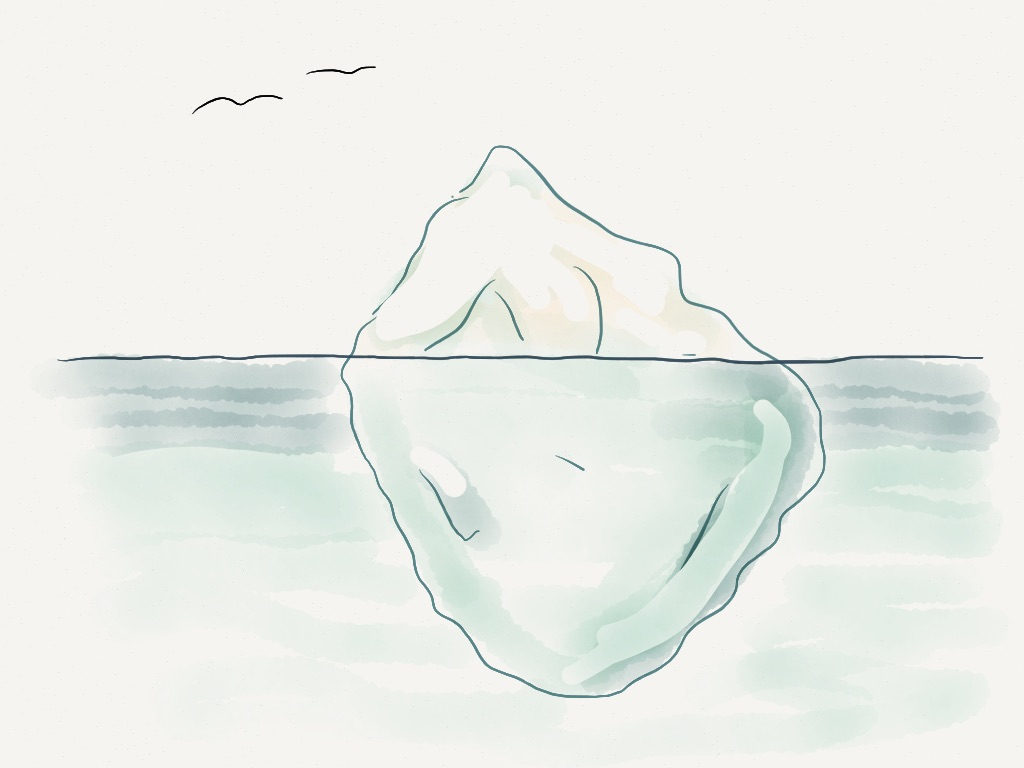
\includegraphics[width=10cm,height=5cm,clip=true]{eisberg}\\
\begin{scriptsize}
\begin{picture}(0,0)(200,60)
       \put(185,165){Main Proof}
%       \put(185,155){Beweis}
       \put(190,103){\rotatebox{15}{Eigenvariables}}
       \put(180,130){\rotatebox{-5}{Hypothesis}}
       \put(230,127){\rotatebox{5}{Variables}}
       \put(242,120){\rotatebox{-5}{Context}}
       \put(170,140){\rotatebox{0}{Renaming}}
       \put(202,90){\rotatebox{25}{Derivation Tree}}
       \put(180,115){\rotatebox{5}{Substitution}}
       \put(220,140){\rotatebox{5}{Scope}}
       \put(250,140){\rotatebox{-5}{Binding}}
\end{picture}
\end{scriptsize}
  \end{center}
  \caption{Proofs: The tip of the iceberg}
  \label{fig:iceberg}
\end{figure}

To visualize the overhead involved, consider Fig.~\ref{fig:iceberg}. Above the water is the main part of the proof, which is often fairly straightforward. However, when mechanizing formal systems we also need to implement bound variables and their scope, work modulo renaming of variables, keep track of and manage lists of assumptions and enforce properties about them, and define substitution together with its equational theory, among other things. Early work \citep{Berardi:WLF90,CCoquand:92,Altenkirch:TLCA93}  within general purpose proof environments represented lambda-terms using (well-scoped) de Bruijn indices, which leads to a substantial amount of overhead to prove properties such as substitution lemmas and composition of substitution.
To improve readability and generally better support such meta-theoretic reasoning, nominal approaches support $\alpha$-renaming but substitution and properties about them are specified separately; the Isabelle Nominal package \citep{Urban:JAR08} has been used in a variety of logical relations proofs from proving strong normalization for Moggi's modal lambda-calculus \citep{Doczkal:LFMTP09} to mechanically verifying the meta-theory of LF itself\unsure{this is the first mention of LF, so maybe not ``itself'', or some mention of it earlier? -am}, including the completeness of equivalence checking \citep{Narboux:LFMTP08,Urban:TOCL11}.  However,  these approaches still lack the right level of abstraction. It should not matter how we implement variable binding, contexts and substitutions -- rather, users should be able to use these concepts first-class.
% One might compare the situation we face to a programming language  lacking abstract data types i.e. the power to abstractly define values together with operations on them.  %  As a consequence, these developments lack important aspects: flexibility (we cannot easily change the representation of substitutions or variables).

\beluga~\citep{Pientka:IJCAR10,Pientka:CADE15} follows this path and provides a sophisticated infrastructure to automatically deal with many bureaucratic details regarding variables and  assumptions, while giving up  (at this point) some of the computational power present in general proof assistants such as Coq and Agda.  We harness the power of abstraction, by defining common concepts such as variable binding and derivations depending on sets of assumptions together with sets of operations and properties. While these concepts, their operations, and their properties are grounded and carefully defined theoretically, users do not need to understand any technical details on how these concepts are implemented nor do they need to prove (often standard) lemmas;  instead they simply use these concepts abstractly through the syntactic constructs provided. As a consequence, mechanizing proofs about formal systems, even advanced proofs by logical relations, does not require a deep and complicated mathematical apparatus, but can be carried out in a direct and intuitive way.  In fact, the proof language used for developing the main proof (i.e. what is above the water) is a proof term language for first-order logic with induction over contexts and derivation trees (objects that are first-class). In essence, \beluga's proof language is comparable to first-order logic with induction over a specific domain --- in our case the domain must be rich enough to allow us to describe derivation trees that may depend on assumptions. By doing so we harvest many of the same benefits that abstract data types bring to programming languages \citep{Liskov:74}: we can change the concrete representation implementation of variables, substitutions, and contexts, choosing what is most efficient;  proof developments are modular and as users do not have direct access to the concrete implementation of variables, substitutions, and contexts, they also cannot add any tempting, but dangerous shortcuts that would corrupt part of the infrastructure; and most importantly, proof developments are easier to understand and read, as the high-level steps are not obscured by low-level operations, and as a consequence, we stand a chance to automate such proofs.

In this exposition, we introduce \beluga by example, starting from a simple language of arithmetic expressions (as described for instance in \cite[Ch 3, Ch 8]{TAPL}) and showing how to encode this language together with simple inductive proofs  in \beluga. This will allow us to introduce the basic idea of encoding proofs as recursive functions. We then extend our simple language of arithmetic expressions to include functions (as for example described in \cite[Ch 5, Ch 9]{TAPL}). This introduces several important ideas: how to encode variables and their scope, how to encode assumptions, and how to characterize derivations that depend on assumptions. Finally, we consider the proof of normalization for the simply typed lambda-calculus (see \cite[Ch 12]{TAPL}) and show how to directly represent this proof as a recursive program in \beluga. Throughout the text we will point to exercises that allow readers to practice and explore some topics further.

\paragraph{Words of wisdom}
We do not give a formal definition of \beluga's language.  Instead,  we look at examples and highlight how to \emph{use} \beluga rather than dwelling on how it is defined. This is in fact how most learn a given programming language --- a language is best learned by using it. We believe learning \beluga is best approached with a blank state of mind. Try not to compare it to functional languages you already know. While \beluga is a functional language and has even a similar syntax to OCaml,  it requires a different way of thinking about programming than what you have been acquainted with when using OCaml or ML.


% \paragraph{Know where you are from and where you are going} \beluga builds on and extends many ideas developed in the logical framework, \twelf \cite{Pfenning99cade}.

\section{Goals}
We pursue several goals with this companion:

\begin{enumerate}
\item Understand how to define formal systems using higher-order abstract syntax
\item Curry-Howard isomorphism: Proofs = Programs
\item Deeper understanding of programming languages and their properties
\item Provide a tutorial to \beluga
\end{enumerate}


% \section{Mechanizing Definitions} Language formalization frequently
% start an informal, on-paper definition of the language. It mostly
% consists of 3 distinct parts:

% \begin{itemize}
% \item Represent the grammar / syntax of a language
% \item Represent its operational and static semantic
% \item Represent its meta-theory, i.e. proofs about the semantics such
%   type preservation and progress, correctness of program transformations, and normalization.
% \end{itemize}

% Each layer brings up different questions we must address. The choice
% we make in each of the questions substantially influences how easy it
% is to attack the next layer.  There are a number of systems we could have chosen to mechanize each layer such as Coq or Isabelle. In these notes we use system that is specialized for our task and provides the most supporting infrastructure.


% \section{Adequacy} An important question we must keep in mind in
% this endeavour is the following:
% What does it mean to correctly represent such a language
% definition in a formal framework? -- In general, we aim for a
% \emph{adequate representation}, i.e. the objects represented formally
% in the framework describe exactly those we were talking about on
% paper. More precisely, the representation of the language is
% isomorphic to the informal definition of the language we had on
% paper. But in practice we even want more: we want that the structure
% of the language is preserved as well -- this will mean that we want a
% bijection (in fact a compositional bijection).

% To establish adequacy, we require two tools: 1) Adequacy proof:
% induction proofs on the canonical forms of LF 2) Modularity of
% adequacy proofs based on subordination (we must understand under what
% assumptions/circumstances is an encoding adequate and when it is
% adequate with respect to one set of assumptions, how do we know it
% remains adequate given some other set of assumptions)

% Adequacy is a deep property of an encoding and maybe surprisingly it
% is a property that often does not hold. In fact, often our
% representation in some programming / proof environment admits many
% more terms than are meaningful.

% We omit here a detailed discussion of how to prove adequacy, we
% will refer the interested reader to the article
% \citep{HarperLicata:JFP07}.

%%% Local Variables:
%%% mode: latex
%%% TeX-master: "book"
%%% End:
